% vim: set tw=79

\documentclass[a4paper,10pt]{article}

\usepackage[utf8]{inputenc}
\usepackage{lipsum}
\usepackage{a4}
\usepackage[inline,nomargin]{fixme}
\usepackage{amsmath}
\usepackage{amssymb}
\usepackage{graphicx}
\usepackage{grffile}
\usepackage{url}
\usepackage{hyperref}
\usepackage{xcolor}
\usepackage{colortbl}
\usepackage{chngcntr}
\usepackage{caption}
\usepackage{subcaption}

% Python listing setup

\usepackage{color}
\usepackage[procnames]{listings}
\usepackage{textcomp}
\usepackage{setspace}
\usepackage{palatino}
\renewcommand{\lstlistlistingname}{Code Listings}
\renewcommand{\lstlistingname}{Code Listing}
\definecolor{gray}{gray}{0.5}
\definecolor{green}{rgb}{0,0.5,0}
\definecolor{lightgreen}{rgb}{0,0.7,0}
\definecolor{purple}{rgb}{0.5,0,0.5}
\definecolor{darkred}{rgb}{0.5,0,0}
\lstnewenvironment{python}[1][]{
\lstset{
language=python,
basicstyle=\ttfamily\small\setstretch{1},
stringstyle=\color{green},
showstringspaces=false,
alsoletter={1234567890},
otherkeywords={\ , \}, \{},
keywordstyle=\color{blue},
emph={access,and,as,break,class,continue,def,del,elif,else,%
except,exec,finally,for,from,global,if,import,in,is,%
lambda,not,or,pass,print,raise,return,try,while,assert},
emphstyle=\color{orange}\bfseries,
emph={[2]self},
emphstyle=[2]\color{gray},
emph={[4]ArithmeticError,AssertionError,AttributeError,BaseException,%
DeprecationWarning,EOFError,Ellipsis,EnvironmentError,Exception,%
False,FloatingPointError,FutureWarning,GeneratorExit,IOError,%
ImportError,ImportWarning,IndentationError,IndexError,KeyError,%
KeyboardInterrupt,LookupError,MemoryError,NameError,None,%
NotImplemented,NotImplementedError,OSError,OverflowError,%
PendingDeprecationWarning,ReferenceError,RuntimeError,RuntimeWarning,%
StandardError,StopIteration,SyntaxError,SyntaxWarning,SystemError,%
SystemExit,TabError,True,TypeError,UnboundLocalError,UnicodeDecodeError,%
UnicodeEncodeError,UnicodeError,UnicodeTranslateError,UnicodeWarning,%
UserWarning,ValueError,Warning,ZeroDivisionError,abs,all,any,apply,%
basestring,bool,buffer,callable,chr,classmethod,cmp,coerce,compile,%
complex,copyright,credits,delattr,dict,dir,divmod,enumerate,eval,%
execfile,exit,file,filter,float,frozenset,getattr,globals,hasattr,%
hash,help,hex,id,input,int,intern,isinstance,issubclass,iter,len,%
license,list,locals,long,map,max,min,object,oct,open,ord,pow,property,%
quit,range,raw_input,reduce,reload,repr,reversed,round,set,setattr,%
slice,sorted,staticmethod,str,sum,super,tuple,type,unichr,unicode,%
vars,xrange,zip},
emphstyle=[4]\color{purple}\bfseries,
upquote=true,
morecomment=[s][\color{lightgreen}]{"""}{"""},
commentstyle=\color{red}\slshape,
literate={>>>}{\textbf{\textcolor{darkred}{>{>}>}}}3%
         {...}{{\textcolor{gray}{...}}}3,
procnamekeys={def,class},
procnamestyle=\color{blue}\textbf,
framexleftmargin=1mm, framextopmargin=1mm, frame=shadowbox,
rulesepcolor=\color{blue},#1
}}{}



\counterwithin{figure}{subsection}

\setlength{\parindent}{0.0in}
\setlength{\parskip}{0.1in}

\newcommand{\varopt}[1]{\textsc{#1}}
\newcommand{\numbots}{4}
\newcommand{\foodmass}{0.05}
\newcommand{\lightintensity}{0.01}

% Warning: these two are tightly coupled!
\newcommand{\tickinterval}{100 ms}
\newcommand{\tickspersecond}{10}



\title{
    IT - 3708 Sub-Symbolic AI Methods \\
    Homework Exercise 4\\
    ~\\
    \emph{A Controller for Swarm Behaviour in Webots}
}
\author{
    Edvard K. Karlsen \\
    \texttt{edvardkk@stud.ntnu.no}
    \and
    Magne Vikjord \\
    \texttt{magnevan@stud.ntnu.no}
    \and
    Jonas Asmundsen \\
    \texttt{jonasbal@stud.ntnu.no}
}
\date {}


\begin{document}

\maketitle

\section{Introduction}
In this project we will design a controller based on Brooks Architechture to
explore cooperative transport of a box in Webots environment. Intended box
pushing task draws inspiration from swarm behaviour of ants observed often
during food retrieval. The idea is to create a decentralized system invoking
group behavior through simple mechanisms which if successful, leads to an
emergent self-organized behaviour.

The rest of this report is structured as follows. In Section~\ref{sec:a1} we
give a brief overview of our system (Deliverable A1).  Further, in
Section~\ref{sec:a2} we describe our control system, and discuss its observed
behavior (Deliverable A2). Then, in Section~\ref{sec:b1} we discuss possible
improvements to the system (Deliverable B1). Finally, in Section~\ref{sec:b2}
we present out implementation of the improvements, and discuss how they
improved the e-puck's performance in the simulation (Deliverable B2).

\section{System overview}
\label{sec:a1}

\subsection{Changes to world}
We tried to emulate our world to behave as closely to the live demonstration
we were given of the e-pucks swarm. Thus, we made the following changes:

\begin{itemize}
    \item Removed all loose solids from the world except for one, which will
    become our food.
    \item Added physics to the food, and set the mass to \foodmass.
    We found this to be a good number for our basic tests as it
    requires two or more bots to be cooperating to push the box.
    \item Added a point light to the food with intensity \lightintensity.
    \item Removed all ambient lighting, and all other point lights. (Thus, the
    only remaining light source is the food.)
    \item Increased the number of e-pucks to \numbots.
    \item Reduced the tick interval to \tickinterval.
\end{itemize}

\clearpage

\section{E-puck control system}
\label{sec:a2}

The arbitrarian component of a subsumption-based system can be implemented in
many ways, from ad-hoc solutions with explicit, highly coupled,  communication
between layers, to general network graphs with arbitrary supression edges. We
chose a compromise between simplicity and flexibility: we use a single list of
control layers sorted by ascending sophistication. Each time we choose an
action, we iterate through the list of layers, and choose the action proposed
by the most sophisticated supressing layer (or the most primal action, if no
higher layers opt to supress). 

The following Python-style pseudo code shows the outline of the
bot's control system (see \texttt{botty.py}).

\begin{python}
def run_botty(self):
    self.layers = [
        SearchLayer(),
        RetrievalLayer(),
        StagnationLayer()
    ]

    while True:
        self.tick()

def tick(self):
    proximities = self.get_proximities()
    lights      = self.get_lights()
    speed       = self.get_speed()

    output = None
    for each layer in self.layers:
        proposed_output, should_supress = layer.act(proximities, 
                                                    lights, speed)

        if output is None or should_supress:
            output = proposed_output

    self.move_wheels(output)
\end{python}

As is seen, each layer implements a general interface: 
\begin{python}
def act(self, proximities, lights, speed):
    # return two-tuple 
    # (output power), should_supress
\end{python}


\begin{figure}
  \centering
  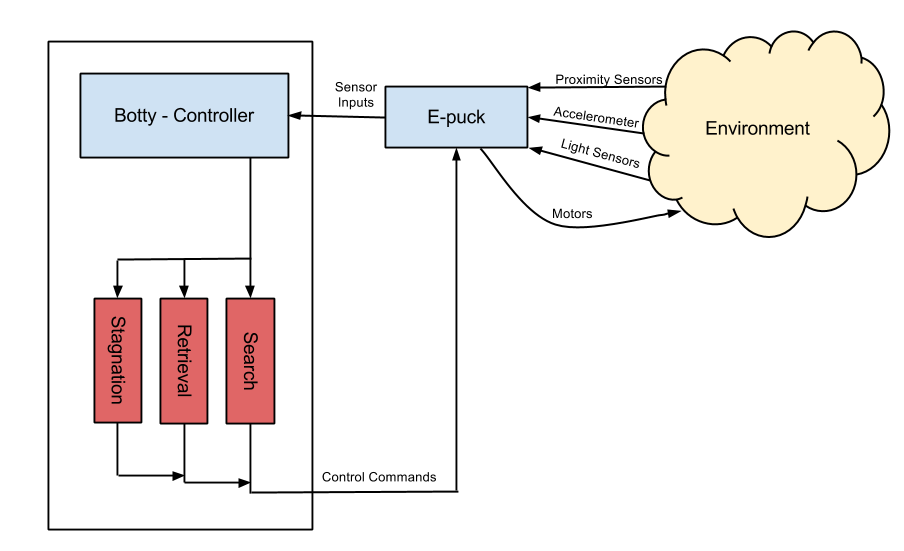
\includegraphics[width=0.8\textwidth]{%
    models/SubSym Proj 4 architecture.png}
  \caption{Controller architecture for the box pushing task.}
  \label{fig:architecture}
\end{figure}

We used the three-layer approach which was used for CRABS, and presented in
the assignment text, but we rewrote each layer from scratch.

\subsection{Search}
The search layer is built as a simple state-based random explorer, which also
tries to avoid crashing into walls.  This layer never suppresses (as it is the
most primitive). 

The exploration function is functionally similar to the following pseudo-code:

\begin{python}
def find_speed(proximities):
    prox_right, prox_left = proximities[:3], proximities[5:]

    # Check for obstacles
    if any(p > DIST_THRESH for p in prox_right+prox_left):
        tot         = sum(prox_right + prox_left)
        left_power  = sum(prox_left)  / tot
        right_power = sum(prox_right) / tot
        return left_power, right_power
    else:
        # No obstacles, continue in set random direction,
        # or, with random probability, choose a new direction
        if random() < PROB_CHANGE_DIR:
            self.rand_move_dir = (
                uniform(.5, 1.0), 
                uniform(.5, 1.0)
            )
        return self.rand_move_dir
\end{python}

The gist of the code is: If there are obstacles nearby, the bot should try
to avoid them. Otherwise, it will just continue in a set random motion, with
some chance of choosing a new direction (with our current parameter choice, a
direction change can be expected after 2-3 seconds). 

\subsection{Retrieval}
The retrieval layer mainly uses the light sensor to detect the presence of a
food source nearby, which when detected, it will home in on, and push.

The retrieval layer will begin suppressing as soon as it detects a light
signal over a certain threshold. When light is detected it will rotate clockwise until 
the light is the strongest right in front of the robot (presumably that's where 
the food is), and then move straight ahead to push it.

\subsection{Stagnation}
The stagnation layer is tasked with identifying stagnation, which is when a 
bot is trying to push a target, but for some reason fails to do so and does 
not move. The method for deducing whether or not this has occurred utilizes 
all sensory value input available.

The layer will collect all sensory input values from the last 
{\tickspersecond} iterations.  

For each sensor, its {\tickspersecond} values are analyzed. If the difference 
between the maximum value of the sequence and the minimum value of the 
sequence is above a certain threshold, stagnation is not considered to be in 
effect. Stagnation will only occur if no sensor reports any significant change 
in value within the {\tickspersecond} most recent iterations.

The following pseudo-code shows this:

\begin{python}
def _has_stagnated(self):
    if len(self._prev_observations) < 10:
        return False

    (proximity_observations,
     light_observations,
     acceleration_observations) = zip(*self._prev_observations)

    # See if proximity has changed in recent future
    if any(abs(max(i_sensor_obs) - min(i_sensor_obs)) > 150
           for i_sensor_obs in zip(*proximity_observations)):
        return False

    # See if light has changed in recent future
    if any(abs(max(i_sensor_obs) - min(i_sensor_obs)) > 150
           for i_sensor_obs in zip(*light_observations)):
        return False

    # See if acceleration has changed in recent future
    if any(abs(max(i_sensor_obs) - min(i_sensor_obs)) > 0.1
           for i_sensor_obs in zip(*acceleration_observations)):
        return False

    # Nothing has changed in recent future
    # This is indicative of a stagnation
    return True
\end{python}

\subsection{Resulting behavior}

Using this system, the robots will often manage to push the box into one of
the corners, as seen in the timings in the table below. However our bots did
display some strange behaviors we might want to correct.

First of, our bots would sometimes loose sight of the box it it was
pushing near the corners of the box, or close to another bot. The result would
be that the bot would sometimes spin almost $360^\circ$ around, instead of
just making the small correction necessary. Another problems was that the
bots would in addition to pushing the food, push each other quite aggressively,
which seems to have at least two detrimental effects.
\begin{enumerate}
\item They would push
each other off the box, which both slows down progress, and sometimes
leads to a change in direction of the box. Sometimes the box would almost
make it to an edge before the robots would make a turn and start pushing
it towards another far away edge.
\item Often we couldn't adequately detect stagnation, because even if
the box itself was not moving, the robots would be nudging each other
continuously, which to our stagnation algorithm is equivalent to genuine
movement of the box.
\end{enumerate}
\item By pushing with an angle and not directly towards the target, some of 
    the force exhibited by the bot is wasted on moving along it. With each bot 
    exerting a reduced amount of force on the target, more bots are necessary 
    to make it move.

\begin{table}
    \begin{tabular}{llllll}
    Run \# & 1     & 2     & 3     & 4          & 5     \\ \hline
    Time  & 00:44 & 00:22 & 00:38 & STAGNATED! & 01:12 \\
    \end{tabular}
\end{table}


\section{Possible improvements}
\label{sec:b1}

\subsection{Aimed retrieval}

The retrieval layer works by rotating until it has determined that it is 
facing the target box. Once it faces the target, it will commence moving 
farward as long as it determines it is still facing the box. The problem with 
this is that the bot will rarely push directly on the box, but with an angle.  
This is not beneficial, as not all potential force is directed towards it.

We have solved this with a technique which controls the motors and the 
direction of the bot by utilizing the two most-front light sensors. This 
technique will make sure that the bot is facing the light source is a highest 
possible degree. The following pseudo-code shows this:

\begin{python}
right, left = float(proximities[0]), float(proximities[7])

if max((right, left)) > DIST_THRESH:
    total = right + left
    l_wheel_speed, r_wheel_speed = left / total, right / total
else:
    l_wheel_speed, r_wheel_speed = 1, 1
\end{python}

\section{Implementating and evaluating the improvements}

\begin{figure}[!h]
    \centering

    \begin{subfigure}[!h]{0.45\textwidth}
        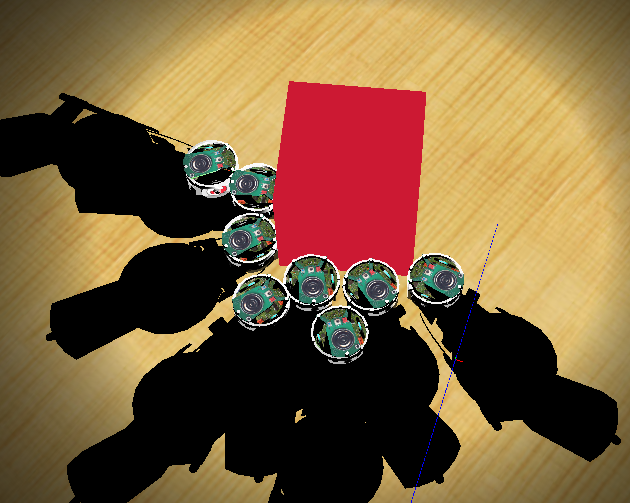
\includegraphics[width=\textwidth]{models/stresstest.PNG}
    \end{subfigure}
    \begin{subfigure}[!h]{0.45\textwidth}
        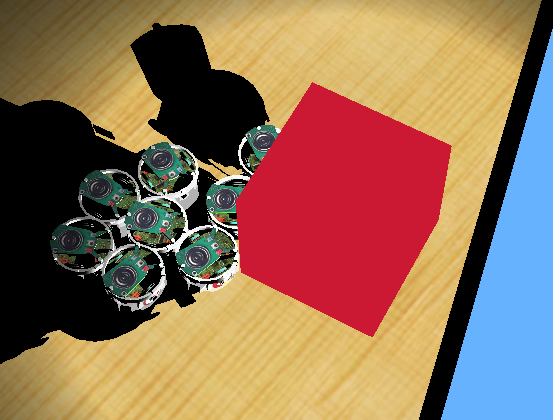
\includegraphics[width=\textwidth]{models/stresstest2.PNG}
    \end{subfigure}

    \caption{A group of eight e-pucks solving a $0.7$-mass box pushing task.
    To move a box with this mass, almost all the robots must take part in the
    pushing motion, and no robot can hinder it.}
\end{figure}


\label{sec:b2}


\end{document}
